%%%%%%%%%%%%%%%%%%%%%%%%%%%%%
% FOWLER
%%%%%%%%%%%%%%%%%%%%%%%%%%%%%
\section{Fowler [better name needed!] \label{sec:fowler}}

This section discusses the work of Christopher Fowler, who has attempted to recreate the \gls{coremodel} in agent form. The issues Fowler discovered in doing this are a perfect primer for the sections that follow. 
%Why interesting? Are the core model issues so fascinating?

Fowler firstly attempted to take the core model out of its equilibrium assumptions; an agent approach, he argues, is a good method for achieving this. He set himself a specific goal: to ``re-create as exactly as possible the relationships in the economic [core] model'' (\citealt{fowler_taking_2007} p.266) in agent form, meaning that ``to the extent possible, the equations used to express the analytic model have been maintained.'' (p.272) Fowler's direction of travel, then, is very much from the analytic core model towards agent modelling. For instance, he keeps the final set of simultaneous equations outlined in section \ref{sec:coremodelapx}. The main conclusion from his first attempt was that -

\begin{quote}
``although the equations of the analytic model can be mimicked in a way that is sufficient for a simulation to run, such a simulation cannot be made logically defensible without significantly altering the relationships among workers, firms and cities posited in the analytic model.'' (p.282)
\end{quote}

In initially binding himself to the assumptions of the analytic core model, Fowler was stuck with one of the more thorny abstractions: there are no firms explicitly defined. The equilibrium number of firms - a key feature of of the Dixit-Stiglitz \gls{monocomp} approach, as discussed in section \ref{sec:marketstructure} - is purely a consequence of consumer demand combined with love of variety. As he puts it, ``firms appear and disappear in cities based on the full employment of the workforce even to the point of following the lead of workers who move from place to place in order to benefit from increased real wages.'' (\citealt{fowler_finding_2010} p.2) 

%\citealt{fowler_taking_2007} defined firm agents, but in sticking with the analytic model's method, did not build any mechanism for matching firms to workers. Following their own motivations, ``when firms move, they tend to want to move to places where wages are low; in contrast, workers tend to want to locate where wages are high'' (\citealt{fowler_taking_2007} p.276). 

Fowler's first pass at an agent version of the core model, then, lacking any method for linking firm and consumer behaviour even implicitly, could not produce equilibrium firm levels. Fowler notes that ``as a result, the model fails to move towards any of the equilibrium conditions predicted by its analytic counterpart.'' (p.266) In his second paper, Fowler attempts to address this by defining mechanisms, having already identified a set of criteria:

\begin{quote}
``firms would bid for labor through wages and set prices for their goods at a level where they would expect to make the greatest profit. Workers would then consume based on the available prices and quantities; utilities and profits could be calculated for all agents. What sets this type of specification apart, however, is that it would make no assumptions about individual firms making the correct choices. Firms that chose correctly would be rewarded, and those that chose poorly could be dropped from the model.'' (\citealt{fowler_taking_2007} p.280-1)
\end{quote}
%The equations for things like production and wage would be truly independent rather than derivative so the model could handle a wide range of parameter configurations. 
%Actors with motivations, mechanisms connecting them and a variety of assumptions about the dynamics that these two together will produce. Fowler suggests some of the mechanisms that a full agent version of the core model might do: 

This is a fully agent-based picture he paints: each actor making decisions entirely independently, based on the information at their disposal. In a statement he later appeared to regret, Fowler goes on to say, ``as complex as this specification sounds, it is actually relatively simple in an agent-based framework where bounded rationality, learning by doing and other types of decision-making all have substantial supporting bodies of literature.'' (ibid.) The reality of building such a model proved less simple. The problem has two components: first, how actors make decisions; second, whether they can collectively coordinate their actions into globally desirable economic outcomes. That, in a nutshell, is the `general' problem in general equilibrium analyses. 

Fowler discusses some of the dependencies that must be solved if an agent model is to work: ``the amount a firm can offer in wages is dependent on the amount it can produce and the price it receives for its goods. These quantities are affected, in turn, by consumer's wages, which depend on which firm employs them (and whether or not they have found employment at all.)'' (\citealt{fowler_taking_2007} p.277) 

Creating a functioning agent model of work and consumption can often involve making coding compromises. Fowler's approach to consumption reflects this: a tactical choice is made that avoids the need to consider rationing of limited goods. As Fowler puts it, ``workers select their optimal bundle of goods without reference to the actual supply of the good.'' (f2 p.10) Thus, they still have an `objective' demand level. He notes a key informational advantage: this sends ``clear signals to firms about the actual level of demand for their goods at the current price'' (ibid.) 
%I do the same currently: infinite stock. 

This reflects the prime difficulty of producing coordination in an agent model of this sort. A proponent of the analytic approach to the core model might argue that this demonstrates the power of the analytic method, but this misses the point Fowler's work has made. Just because dynamics of coordination are hidden behind equilibrium assumptions does not mean they have gone away. It is still very much an open question: how can actors, unable to coordinate through any central mechanism, produce stable spatial economic outcomes? Indeed, is there a model than can achieve this, or are there reasons to believe it might not be possible?
%Referring to the metis arg here. Analytics may describe and endpoint, but the metis argument rules out being able to produce a model of the process. Discuss!

Notes the 'absence of rational expectations' (p.275) - ``The firm and worker agents have perfect information in the sense that they can know the outcomes of their decisions up to a point, but the simulation environment is dynamic and the conditions that they observe at the time they decide where to move will not remain constant as other firms and workers make their own decisions.'' (p.275) Discussed much here in relation to what rationality means in an agent context. Do my blind agents, able only to know when a random grop improved their lot, count as rational?

Later: ``To create such a model, firms would have to have some mechanism with which they could predict an appropriate production level for themselves and estimate the levels chosen by their competition in an environment where sufficient labor supply is not guaranteed. The delicate balance among the equations of the analytic model does not allow for the error and uncertainty that are necessary parts of this sort of prediction, and so a new set of relationships needs to be specified.'' (p.282)
He notes that analytic choices made to gain tractability can ``actually make the problem less tractable'' in an agent setting. (p.283)

%%%%%%%%%%%%%%%
% Fowler 2
%%%%%%%%%%%%%%%
Fowler's goal is still to find optima in his model: he wants to ``explore the capacity of an economic system to identify a stable Nash Equilibrium without it being enforced by assumption.'' (\citealt{fowler_finding_2010} p.14)%Nash eq reminder: everyone's found a strategy that they wouldn't want to change if they can see what everyone else is doing. 

%Fowler's little summary of the core model: ``the effects of economies of scale, the role of preferences for variety in driving trade between regions, and the push/pull relationship between these two factors in shaping patterns of agglomeration and dispersal in economic activity based on transportation costs.'' (f2 p.2)

%``The research presented here maps out, as nearly as possible, the differences and similarities between the behavior of the agent based model and its deductive counterpart.'' f2p.3: gotta be good for me to bounce off. 

His idea of leakage: defined as the difference from the analytic optima. Which is interesting, for comparison, but my version of things is so far from the original, that sort of comparison isn't really feasible. It is also buys into the idea that the objective optima described by the core model do indeed exist. Or perhaps not: his goal is explicitly a comparison. If the goal instead is, starting with ABM, to ask, how to answer these questions?%Whoa, what an awful sentence!

``leakage is not necessarily a weakness of the agent-based model, but an explanation for how suboptimal outcomes may propagate in real systems.'' (f2 p.3) Sequence is important here, who gets to act first. Also, I haven't seen him really discuss that GE already deals with suboptimal outcomes: equilibria don't need to be optimal. But are they suboptimal for different reasons? And do those differing reasons have very different implications for what we should believe about the real world?

Leakage, he argues, comes from using `indivisible agents' (later he says firms can only hire whole people, rather than amounts of time) and differences between agents making simultaneous vs sequenced decisions. There's not much on that here, so plenty to play on. 

%To fulfill its basic objective the model is designed to ascertain when conditions are in equilibrium (when supply equals demand) and when that equilibrium is stable. To do this the model calculates the total supply and the total demand on each turn. When demand is within 1\% of supply, the model is considered to be in equilibrium and a counter starts to record the values for total supply and demand. If these values remain constant through 100 turns, then the model is considered to be in a stable equilibrium and halted. If no equilibrium is identified after 3000 model steps, then it is assumed that no stable equilibrium will be found for this model. (F2 p.14)

%``The complexity of the equations necessary to specify a relationship between the supply and demand for labor is a persuasive argument for the use if a simplifying assumption such as general equilibrium. However, this complexity points to the significance of the issues overlooked when full employment and optimal distribution of firms are assumed rather than aspired to.'' (F2 14-15)
%Yes, that's a point I've been trying to make: simplifying can hide complexity, but it's still there. However, cf. UNSW stand, when does it matter? It's not automatically true that complexity should be included.

%%%%%%%%%%%%%%%%%%%%%%%%%%%%%%%%%
% Equilibrium
%%%%%%%%%%%%%%%%%%%%%%%%%%%%%%%%%
\subsection{Equilibrium \label{sec:equilibrium_n_agents}}

The problem of markets clearing in space... cf bullock, networks. Fowler: ``Equilibrium is the point in system space where supply equals demand, markets clear, efficiency reigns and overall welfare is maximized.'' (p.267) 

(Ladley bullock paper, unpublished AFAIK: The effects of market structure on a heterogeneous evolving population of traders. No other references: they just briefly mention trading in space can't fit into auction model.)
\fixref{ladleybullock}

Hmm: this is an interesting effect of space, isn't it? If all actors are making market decisions on the head of a pin, an auction-style clearing market presents itself as the natural way to think about it. But as soon as actors have location, that becomes impossible. In a situation where production costs are the same for all actors, nearest actors will automatically take precedence.

Points out that equilibrium means being able to set some equations to zero, and set some rates of change equal to each other. [267]

Bring in physical example. Probably needs own section?

Nice quote to bounce off: ``As a rule, geographers have less faith in the importance of equilibrium values for understanding how an economy works.'' (p.271)
Someone who did think them important - as both Krugman and Isard argue, though Krugman not in any depth: we don't believe they exist in the real world, only that the real world tries to reach them. It never succeeds, but in understanding the equilibria, we can understand the processes of change that are going on in the real economy.
Gosh, that was a good summary, I'll have that! Note: Fowler goes on to say ``The economy as it has been represented in geography is typically far too chaotic to be considered at rest or to be operating at some market-clearing point where all labor is employed, all production is consumed and utility is maximized (Plummer et al., 1999).'' (p.271-2) Don't know who that ref is, but back to the point I was just making: no-one claims that the real economy will reach a rest point, only that the models help us understand the equilibria it moves towards. Think ball on rubber sheet in high wind.

%%%%%%%%%%%%%%%%%%%%%%%%%%%%%%%%%%%
% CUTTINZ
%%%%%%%%%%%%%%%%%%%%%%%%%%%%%%%%%%%
%The result was that ``workers locate without regard to labour demand in a particular locaiont

%One element in particular that he focuses on is the equilibrium number of firms - a key feature of of the Dixit-Stiglitz \gls{monocomp} approach. As discussed in section \ref{sec:marketstructure}, firms are derived from consumer demand. They have no independent, decision-making existence as such: ``the number of firms is simply a function of the labour required to produce a fixed optimal quantity of goods.'' (p.270) Given that agent modelling demands that firms exist as separate entities, this presents an immediate challenge for Fowler's attempted translation to an agent model. 
%``� the model assumes that the number of firms in a city is defined based on the amount of labour available in that city and the amount of labour necessary to produce the optimal amount of a good.'' (p.271)

%The direction taken by this project goes the other way: start with agents and work towards the concepts used in \gls{ge}.
%... This thesis comes at the problem from the opposite direction, in two respects. 

%He suggests this finding should lead to caution about making any policy claims based on the core model. I rather think it should instead lead to saying: agent models are different from their analytic counterparts, and those differences have to be respected. You cannot build a model of consumers and firms  - with explicit firms - without specifying how they interact. (You could perhaps model agent consumers and deduce firm numbers somehow, without explicitly creating firms as agents�) If the analytic argument about that interaction does not translate, then one that fits with an agent approach must be constructed.

%One reasonable alternative to a set of equilibrium solutions is a model that incorporates bounded rationality and the possibility of error. In this type of model, 
%Later: ``To create such a model, firms would have to have some mechanism with which they could predict an appropriate production level for themselves and estimate the levels chosen by their competition in an environment where sufficient labor supply is not guaranteed. 
%I should try and end up with a list of aspects of interest. So, these are things that ABM particularly draws attention to. To include:
%- how demand should work. Fowler goes for objective budget.
%- mechanisms for: linking production to labour; wages to employment. (So says Fowler.)
%- equilibrium level of firms. The connection between demand andntry/exit

%Hey! The seques nicely into a discussion on equilibrium, doesn't it? Aaawesome-ee-doo-dah!

%\begin{quote}``The logical step to improve the functionality of this model is to develop equations that account for the rationing of wages and production, based on worker employment (for wages) and availability (for production)... the model must be reformulated from its most basic assumptions before such rationing can be incorporated to move forward in this highly desirable direction.'' (\citealt{fowler_taking_2007} p.277)\end{quote}

%This is, of course, exactly the kind of argument Hayek was attempting to counter: success in providing a model rationing system would end up saying nothing about the fundamental problem of how disaggregated actors can coordinate production. There are benefits, however, to the `subjective' approach of testing possible goods bundles against utility, parallel to the benefits of blind search: no prior knowledge of the state of the market is required. Actors can act based on the informatin presented to them.

%Fowler quotes Amin and Thrift calling for a ``move away from the long shadow of economics'' \fixref{(Amin and Thrift 2000)}. Again, the direction of this thesis is actually more towards some aspects of traditional economics. 

%%%%%%%%%%%%%%%%%%%%%%%%
% ACTION AND INTERACTION
%%%%%%%%%%%%%%%%%%%%%%%%
\section{Action and interaction \label{sec:actions}}

Agent models are iterative by default: agents must act in discrete steps imposed by the computational structure of the machine they run on. Given that fact, methods must be employed to design agent models with appropriate timing. This section deals with this point by explaining what choices needed to be made in the development of \gls{modelname}.

Section x argued that agent models should be designed with functional isomorphism in mind, not code isomorphism.
\cmt{`Section x argued that agent models should be designed with functional isomorphism in mind, not code isomorphism.'}
Nowhere is this more true than when constructing the timing inter-relations of the model. Ultimately, the model structure itself cannot do all the work of showing its relation to reality: the modeller must make an argument, with as much clear awareness of the limitations of the method as possible.

What I was trying to say there: there's a grey area with all agent modelling - we want code structures to be capturing some element of reality that we are interested in, as a map does (Scott), but the precise way it does that may be completely implicit. So e.g. Oeffner citing Tesfatsion: hoping to use \gls{oop}'s distinctions between public, private and protected methods may work in some situations, but there are very few solid rules about how code can be claimed to map to the real-world features the modeller is interested in. The `meaning' in data, meaning response is one example. This sort of thinking tool may be more useful than any number of coding structures. So again, the isomorphism between code and theory may also be implicit, rather than hard-coded.

So, relate that back to Friedman.

%%%%%%%%%%%%%%%%%%%%%%
% BASIC TIMING CHOICES
%%%%%%%%%%%%%%%%%%%%%%
\subsection{Basic timing choices}

As already mentioned, a model run `day' is the most fundamental unit of time. Beyond that, the way timing is structured in model scenarios is one of the most important determinants of outcome. How do actors `know' when to take an action? The most common approach \fixref{ref for randomising agent action order?} is to randomise the order of actions. That approach is important to avoid artifacts arising as a result of actor order, but it raises its own problems. Consider a scenario with both firms and people, where all actions are daily randomly permuted, both firms and people mixed. An obvious logical outcome is that the time between any one actors' actions will vary. There is a small probability on each day that two of their actions will actually be consecutive: at the very end of one day and the very beginning of another. That also means, of course, that the subsequent action could be almost two `days' apart. More generally, the time between actions will never be consistent. Why should this be a problem? An example: if a firm is making decisions based on responding to a change in net income between days, it will be based on faulty data. There are two ways around this: firstly, the actions of people and firms can be put into two `bins' and permuted separately. This guarantees that all people will have made market decisions before firms come to act. Second, firms can be allowed to know the length of time between decision points and alter their decision-making (for example, by correcting the rate of change of net income accordingly.)

\cmt{Don't know if I'm including this dynamic yet.}
In the scenario just discussed, each actor acted only once per day. The order was randomly permuted, but that single-action daily limit defined what a `day' was. There may be other stopping conditions that define the boundary of a day, and these may mean an arbitrary number of actions occur. In a clearing market, for example, the day may not be over until all firms have the labour they require, or all people have the wage they want. (Note that, in that situation, firms may end up without having employed all the labour they would prefer, or some people could find themselves unable to work.) Rather than a single action each, this scenario could see actors contacting others many times before one of those two stopping conditions is met.

Often, the importance of timing structure is much less obvious than the random permutation problem. As an example, consider a scenario where people choose wages and goods in the same `moment' (that is, during one action). They will not work if no goods are available, as there is no point: they cannot buy them. Equally, if no work is available, they cannot afford to buy anything. This can lead to a catch-22: if firms run out of stock, they need labour to make more, but no-one will work if no stock is available. This also illustrates a point that will be returned to: is this catch-22 a `bug' or a `feature'? That is, should the modeller be arguing that it says something about the real world, or that the model is broken and needs fixing?

The description of timing, then, will summarise as briefly as possible what particular structure is being used for a scenario. 

\cmt{bug or feature? Where do I discuss that? Also, how to describe timing issue of e.g. changing time input between firm actions? And online vs offline optimisation? That relates to timing but overlaps with action. Relates also to whether actors are facing a `static' world or not... how to tie that together coherently?}

\subsection{Data, meaning, response \label{sec:dmr}}

Stafford Beer: weathervanes - ``it is the wind that is capricious; the measurement does not make mistakes.'' (\citealt{beer_what_2002} p.214)

Different kinds of uncertainty: that one is physical. The measurement is accurate. My agents: having to react to other agents, not knowing how they will respond...?

This section introduces the idea of \gls{dmr}, taken from Jane Jacobs' final book, `the Nature of Economies' (\citealt{jacobs_nature_2001}). In it, Jacobs looks for the common thread that ties supply and demand to other feedback mechanisms in nature. She settles on the importance of integration between `the data, the meaning of the data and appropriate responses to the data.' (p.109) That framework functions, she argues, for systems as disparate as a termite mound, where supply and demand of soldier termites is precisely controlled through distributed pheromone signals, and price data, which can `carry meaningful information on imbalances of supply and demand and automatically trigger corrective responses.' (p.110) That tripartite split - data, meaning of the data, appropriate responses to the data - is very useful for thinking about how to develop agent-based models of economic activity.

%stick the hayek stuff in here: price as a signal cannot be reduced to something simple. It's the end of a process, a summation of carefully won, specialised knowledge: metis.

The slippiest term here is `meaning'. As will be discussed in chapter \ref{chapter:models}, meaning is rarely defined in explicit code form. Rather, the overall code structure is taken to represent meaning for a particular agent. 
\cmt{meaning: rarely defined explicitly? I'll probably end up defining it completely implicitly. If so, come back here and change `rarely' to `never in the models presented here.' Also, I think this issue is discussed in this chapter, and belongs here.}
In-keeping with the overall aim of using as simple assumptions as possible, meaning will be used as narrowly as possible. For example, it is possible for cultural meaning to vary geographically, in economically vital ways. Spedding has an example from cattle markets that illustrates this point nicely: 

\begin{quote}
``Even when good information is ostensibly available, it may not be precise enough. For example, published statistics would suggest that there is a fortune to be made by transporting top-quality Friesian calves from one market in East Anglia to another no more than twenty or thirty miles away. This is not, in fact, the case - it simply happens to be the practice to sell them rather older and heavier in one market than in the other, and in consequence they fetch a somewhat higher price there.'' (\citealt{spedding_freams_1983} p.458)
\end{quote}

This kind of `cultural economic' meaning will be excluded: data will use the same units and have the same metadata assumptions for all actors. 

As in Jacobs, the \gls{dmr} framework should be considered a feedback loop. When considered as a feedback, the simplest form of meaning becomes apparent. An actor takes an action, waits to receive data, and then interprets that data based on that action before responding again. The model in section \ref{sec:firmsLoV} examines exactly this: firms move and then decide if that action was appropriate based on one datum - revenue change. The simplest interpretation of the data - firms' take on its meaning - is, `did my revenue increase? Then the action was a success.' 

%%%%%%%%%%%%%%%%%%%%%%%%%%%%%%%
% COORD N TIMINZ
%%%%%%%%%%%%%%%%%%%%%%%%%%%%%%%
\subsection{The effect of coordination and timing on decisions \label{sec:agenttimings}}


%MM1 30	Big question: 
Is it possible for the model to adjust itself to a situation where working, production and buying is possible? In general, the theory is yes: nominal prices should shift to accommodate demand and underlying utility until it finds a level that works. 
%That's what's generally happened for me in the past, and that makes sense. It's just working out how firms should do this - people don't do any actual adjusting, they merely optimise given prices at the point they act.


MM2 70	Randomness, order of perturbation: how important, what effect? Needs writing up. E.g. choice to separate into two blocks the actions of firms and workers. Why? To make sure the gap between firm decisions is big enough to keep the data sensible. (Because, due to randomness, firms could end up taking two decisions right next to each other, before any person has had a chance to act.)


%%%%%%%%%%%%%%%%%%%%%%%%%%%%%%%
% BLIND SEARCH VS RATIONALITY
%%%%%%%%%%%%%%%%%%%%%%%%%%%%%%%
\subsection{Blind search versus rationality \label{sec:blindvsrational}}

A simple example involves using the basic production function from the \gls{coremodel}: $l=a+bx$. Setting $a=3$ and b to unity, and isolate the expression for the output, $x$, instead, this is just $x=l-3.$. Usually, `average labour' is the focus (which is labour per unit of output; this declines as total labour increases in increasing returns functions.) It is easier to see the role that $a$ - the fixed labour requirement - takes if instead the axes are switched and `output per unit of labour' is the focus. 

\begin{figure}%
\centering
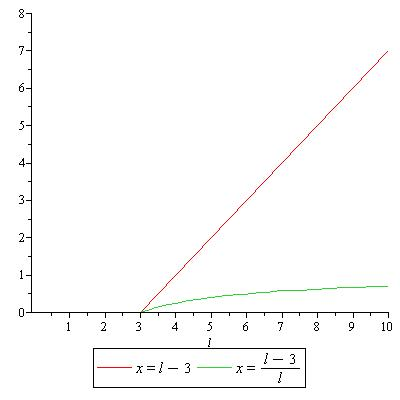
\includegraphics[width=0.5\columnwidth]{ChapterABM/figures/coremodelprodABMjpeg}%
\caption{Core model production function showing total output and average output per unit of labour}%
\label{fig:coremodelprodABMjpeg}%
\end{figure}

Only positive values make sense in an economic context, and as can clearly be seen, the fixed labour requirement means no production is possible at all unless three units of labour are input: an indivisibility. This is straightforward enough to impose analytically, but how might it work in an agent context? The answer is a useful illustration of how rationality, timing and `\gls{blindsearch}' interact. Consider these two possibilities:

\begin{enumerate}
	\item Actors decide sequentially, looking at what firms are producing in order to choose whether to work;
	\item At $t-1$, Actors randomly choose a potential employer. If at $t$ this was successful, they repeat the same action. 
\end{enumerate}

The first of these assumes actors are able to rationally choose a workplace. However, each actor is only able to contribute one unit of labour; a firm needs three to even begin producing. The rational result is that no work takes place and nothing is produced: the model cannot get started. The second is the most rudimentary \gls{blindsearch} possible: attempt some random action at one point in time, and see if it improved things on the next day. If it did, stick with the same strategy. Even with a set of actors consisting of only four people and $n$ firms, given enough time they would all randomly find themselves selecting the same firm and allowing production to take place.

Note, this is not really `blind search versus rationality' as such, since the search requires actors to have the most fundamental attribute required for rationality: to be able to tell `better' from `worse'. 

%WUD 40	Blind search agents: advantage = they have no need to know everything at the same time. Attempts to improve position can be separated out over many timesteps.

%WUD 43	Brute force vs analytic optimisation: catch 22 in actor model where they try to optimise on their time-step: no stock = no point in working; no work = no stock.

%%%%%%%%%%%%%%%%%%%%%
% COMMUNICATING COSTS
%%%%%%%%%%%%%%%%%%%%%
\subsection{Communicating costs \label{sec:comm_costs}}

The first technical challenge is dealing with price. In the \gls{coremodel}, a numeraire approach is used, as described in section \ref{sec:keyconcepts_coremodel}. The `price' of the agricultural good is designated the numeraire. Because output is linear, workers are always `paid' exactly the same. Compare what would happen if numeraire output has increasing returns: output per worker would be higher for larger worker input, and the value of the numeraire would change accordingly. So, any complications regarding agricultural wages are thus done away with. The analytic advantages for the \gls{coremodel} are strong. When it comes to building an agent model with more than one good, however, the numeraire approach is difficult. The existence of agents requires the modeller to specify the relationships between them explicitly: there is no avoiding it. If, for example, two firms each make a different good, and one is the numeraire, each firm must pay wages in that numeraire. How does the non-numeraire firm do this? It must acquire the currency, and can only do this by exchanging what it produces - yet there is no guarantee the numeraire-producers want to exchange. In the basic \gls{coremodel}, for example, no manufacturing output is required to produce agricultural output. An explicitly coded numeraire, then, seems unworkable on the face of it.
%I will try and build one that avoids money, but that's a little way off: it'll be back to collaboration again, plus Edgeworth-like trading.

The use of fiat money solves this problem: all goods and wages can then have a negotiable price. However, a whole set of new challenges accompany the use of money. 


Exchange of information between humans is not the same as for `information' in a computer, or in genes for that matter.  There's a symbolic system: ``The information held and transmitted in the form of a symbol is thus embedded in a network of interconnected meanings, related to and produced by social structures.  Genetic or computer information does not have this quality; it is at most indexical. In contrast, human information is structured and cultural; it is entwined with institutions.'' (\citealt{hodgson_economics_1996} p.253)



\begin{comment}

E.g Eos: (MM2 43) Firms should be able to exploit EoS, but how should that happen? Cf MM1 42 backyard.
MM1 66: firms with higher inputs of labour should have an advantage - they should be able to find a better price than others, if they're ahead; they should have able to get a monopoly.

The point there: geneq is meant to do this; account for all those dependencies. Cf. Fowler.

WUD 4	``Although a full description of this alternative is beyond the scope of this article, it appears that the choice of asynchronous rather than synchronous decision-making is not a key point in understanding the differences between the agent-based and analytic models.'' (Fowler 274)
I disagree! Big, complex issue. Order and randomness large effect on outcomes. Maybe not so with Fowler's very small number of agents.

WUD 22	Auctions vs on-line adjustment versus simultaneous eqs. Actors' decisions spread over time = normal.

FDA 16: Trapped in loops of dependency! Where to work, what to buy, who to hire, where to locate? All affect each other. 

Update: I should just note quite how much I struggled with this problem initially. The answers wer far, far from obvious. I have a solution that runs, but a) many more must exist and b) it may run, but does it really work?

Quote from Fowler: ``the amount a firm can offer in wages is dependent on the amount it can produce and price it receives for its goods. These quantities are affected, in turn, by consumer's wages, which depend on which firm employs them (and whether or not they have found employment at all.)'' (p.277)
There's intrinsically a limit on what agents can do to solve these problems. There's game theory: trying to optimise under uncertainty. But it's not a problem of lack of information: it's a problem of incalculability. 
This may mean, also, that - say - the resulting number of firms is due to a random number failing; no way to predict who, but the incalculability of the problem means that only some will make the right guesses. Cf. Baumol quote on what firms should do to optimise.
Also noted here that the landscape itself is a form of memory.

From Oeffner:
Incalculability: p.25. He talks about it in different terms, but it's the same issue: a difference between 'risk' and 'true uncertainty' stemming from the fact that you don't know what other agents are going to do. Ties to data, meaning
'Endogenous uncertainty': Pesaran 1987. On p.27. That's exactly the problem with two firms trying to find a good location. 


FDA 17	Agents deciding when to sell. Fream: farmers releasing goods in a way that smooths prices. Cf. Kirman's argument about the representative agent, and disaggregated models explaining this kind of smoothing.
The point there isn't so much that you can affect demand - you can, but the effect is small - but that you want to adjust your timing to fit with the macro-effect of supply on demand. You can't really affect prices, but you know prices are going to change in a certain way over time. So, you're a price-taker in the short-term, but there's a longer-term strategy that means you have some wiggle-room - so are actually not a price-taker - and the long-term result is a smoothing of prices. Again, Kirman.

WUD 1	Fowler: ``it is impossible for firms to make decisions about production levels without knowing exactly what every other firm will do and where labour will be available.'' (p.265)
But they don't need to: blind groping. 

WUD 1	Common goal of 'perfect information' vs 'groping' agents: optimisation. Question: how important, if at all, is the 'realism' of the agents? Mine aren't at all. One arg: objective existence of optima; nature of agents doesn't matter; disaggregation is the thing. Fowler: : ``Agent-based modeling works by disaggregating the modeling environment to the extent that each firm and agent is represented as acting individually.'' [265]

==
WUD 2	Determinacy, uniqueness, stability. Necessary for equation-based results? ABM: randomness = come up with probabilistic answers. 
WUD 3: Useful quote, Fowler: ``The economy as it has been represented in geography is typically far too chaotic to be considered at rest or to be operating at some market-clearing point where all labor is employed, all production is consumed and utility is maximized (Plummer et al., 1999).'' (p.271-2) No-one claims that the real economy will reach a rest point, only that the models help us understand the equilibria it moves towards. Think ball on rubber sheet in high wind.
Plus, if completely blind agents can find their way "on-line" to optima, that chaos doesn't present a problem. May be too chaotic to be at rest, but not so chaotic that optima can't emerge through blind luck (and not evolution, unless one considers the landscape as an evolutionary memory. If so, it's Lamarkian!)
There must be a trade-off between how much the world is changing and how much blind groping can achieve, and it must relate in some way to this point about equilibria and change. God knows how though.  
Plus, do agents only capable of telling better from worse count as rational?
WUD5: If a model can grope it's way to optima, with agents' only ability being that they can compare 'before' to 'now', what does that say about the economics? I think this: the equation approach is still entirely valid, but perhaps it's not describing micro-motives. Perhaps instead it's illustrating where the optima are and nothing more. The appeal to utility as a mechanism is false: no action is taken to reach that optima.
One might argue against that: if it can be shown that agents can indeed reach those optima through groping (cf. Walras) then we can assume the mechanism and continue to use analytic optimisation. I'd reply: you have to show that the mechanism does, in fact, work. 
update: which is Epstein's point...
==

MM1 8	Granular, on-line, no market clearing to be done. The many many uses of blind groping.
MM1 15	Supply and demand: stochastic, iterative, not 'clearing'.


===
MM1 18-	Write-up of optimisation and GA. Most useful algorithms assume that there will be some correlation between the quality of 'neighbouring' candidate solutions - those close in the space. Genetic algorithms assume that high-quality 'parent' candidate solutions from different regions in the space can be combined via crossover to, on occasion, produce high-quality 'offspring' candidate solutions." [Mitchell GA p.7]
"What is maximising on-line performance good for? Holland's view is clear: the rough maximisation of on-line performance is what goes on in adaptive systems of all kinds, and in some sense this is how 'adaptation' is defined." [124]
On-line performance: stealing that idea. That was previously "live groping!"
Satisficing.
Worth-noting: GAs combined with hill-climbing algorithms often found to work better than GAs alone. [124] Would seem very likely to be the case for my agents. "GAs seem to be good at quickly finding promising regions of the search space, and hill climbers are often good at zeroing in on optimal individuals in those regions." [124]
Cf. MM2 73: "crawling around in utility space, possibly attempting to swim up a too-turbulent stream and not finding their way�"
===
MM1 42	Cf. split decisions of beanworld; separate auctions for work time and bean buying.
MM1 42	Contrast: backyard model, where actors are able to immediately know whether a particular decision will be more productive for them; indeed, the decision can be taken to be the production, it's so simple. Not so here: the EoS necessary to ultimately lower the cost of production can't happen without a number of people working for a firm; yet, that won't happen below a certain critical theshold, or possibly can't happen at all, given the way I've coded it.

MM2 65	Discussion: the more blindly agents can find optima, the more one can say the objectively exist? Cf. fact the agents make the world they're optimising in, so it can't really be objective can it?

MM2 73	Details of person action choice 2, random groping. So, they might try wage - thus producing stock, thus breaking out of catch 22.

MM1 15	The trick: actors deciding "as if" others are still contributing their time. Need to write up, perhaps compare to simple game theory example

===

MM1 41	Stock running out for some firms shouldn't mean they can't hire - if they have the money. Cf 2 optimisation choices and problems.
MM1 42	Does the stock-crash end-of-model problem say anything interesting about the real world? Is it anything like a co-ordination problem? I.e. people want work, firms want to sell goods, catch 22?
Breaking out: letting work happen before stock levels are known. Is this just a practical modelling solution or something about the real world?
MM1 42	Cf. split decisions of beanworld; separate auctions for work time and bean buying.
MM1 42	Contrast: backyard model, where actors are able to immediately know whether a particular decision will be more productive for them; indeed, the decision can be taken to be the production, it's so simple. Not so here: the EoS necessary to ultimately lower the cost of production can't happen without a number of people working for a firm; yet, that won't happen below a certain critical theshold, or possibly can't happen at all, given the way I've coded it.

%%%%%%%%%%%%%%%%%%%%%%%
% Pasted from Framework: belongs here?
%%%%%%%%%%%%%%%%%%%%%%%

\end{comment}

